\chapter{Sensor Configuration Performance Evaluation} \label{chap:proposed_sys}

As previously declared, the present dissertation ultimately intends to develop a reliable method that determines the optimal configuration to minimize the estimation error. For this purpose, it is necessary to employ a complementary mechanism which is able to perform experiments on sensor configurations in order to quantify their performance based on chosen decision parameters.

Therefore, three different methods will be presented in this section as potential tools to be used. Firstly, a theoretical approach will be detailed, followed by a functional exemplification of each process. Lastly, a practical comparison between them will be presented in order to disclose the preferred option for this application. The first two methods are based on the estimates dispersion given by Monte Carlo simulations of a position estimator, namely a geometry based estimator (GBE) and an estimator that assumes a plane wavefront (PWE), while the third is based on the Fisher Information Matrix.

For all methods, the same scenario is considered which is illustrated in \ref{fig:AoA-init}. It is assumed four hydrophones placed in known relative positions in space and the origin of the axis is set on the body of the AUV or an alternative fixed structure. Then $r_i$ is defined as the vector that connects the origin of the axis to hydrophone $i$ and $rr_i$ defines the vector that connects hydrophone $i$ to the acoustic source. The black cross represents the acoustic source which is located somewhere in space. At last, the subtraction of the mentioned vectors is equal to $r$, according to (\ref{eq:sum-vec}), which corresponds to the position of the acoustic source in relation to the origin of the axis.

\begin{eqnarray}
	& r_i = r + rr_i
	\label{eq:sum-vec}
\end{eqnarray}

\begin{figure}[!htbp]
	\centering
	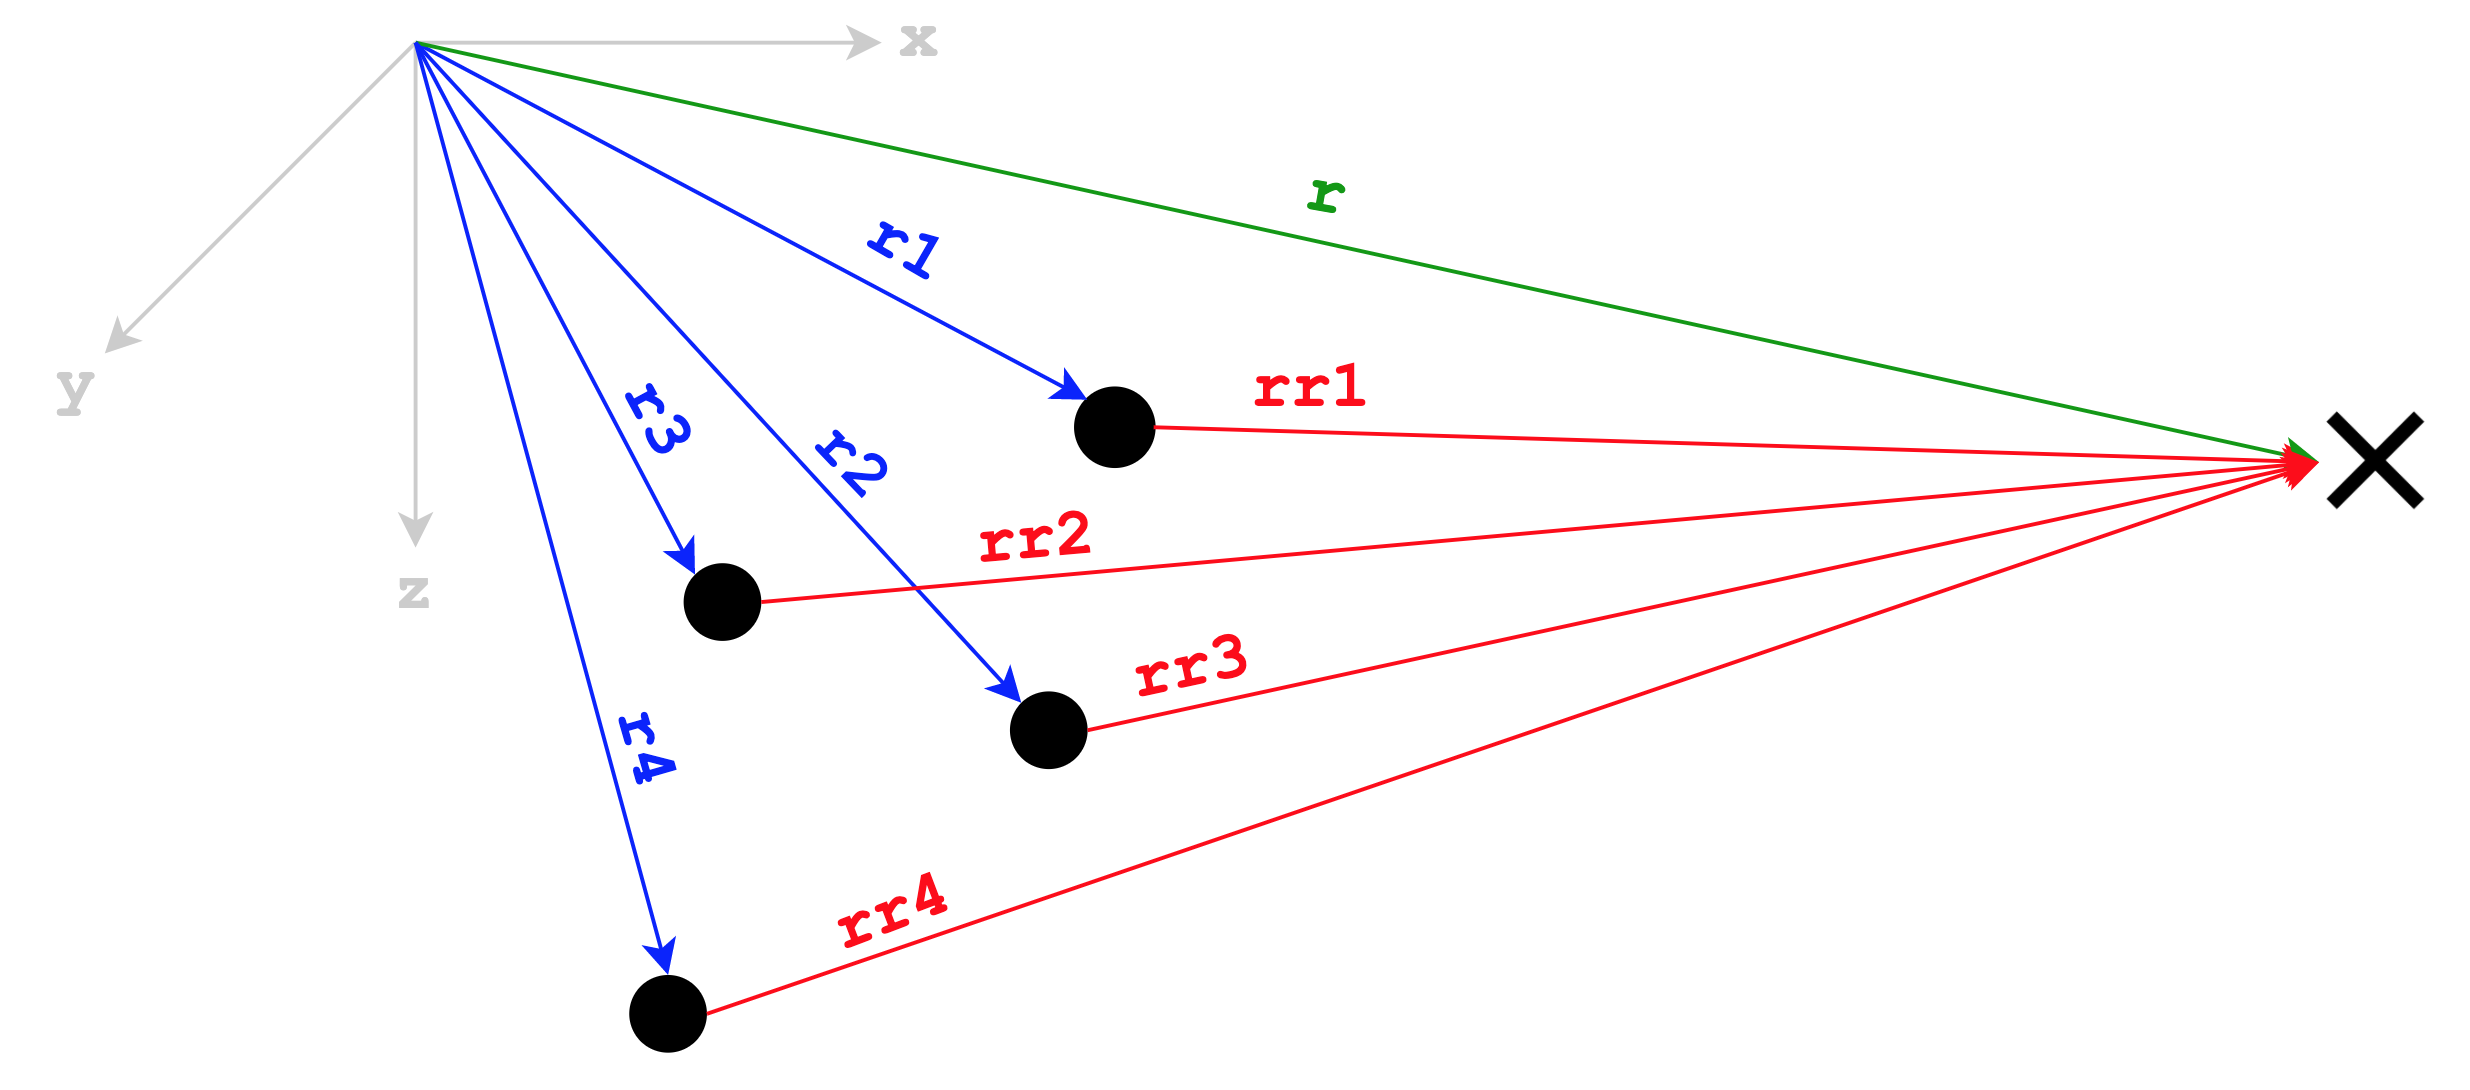
\includegraphics[width=0.8\textwidth]{figures/AoA-init}
	\captionsetup{justification=centering,margin=2cm}
	\caption{Considered scheme for angle of arrival estimation}
	\label{fig:AoA-init}
\end{figure}

%---------------------------------------------------------------------------------
%--------------------------------------------------------------------------------

\section{Geometry based Position Estimator} \label{subsec:estimator}

The goal of the first proposed method is to estimate the position of an acoustic source in relation to known positions of a configuration of sensors, in a system of geometric axes with a defined origin. For this purpose, the logic employed is based on vector algebra with other physical considerations, detailed in the present subsection. 

Considering the presented scenario in \ref{fig:AoA-init}, this explanation starts by defining the times of arrival to each hydrophone, $t_i$ as (\ref{eq:toa-4h}). $t_0$ is the absolute time of emission, $c_s$ is the underwater sound speed and $\rho_i$ is the norm of $rr_i$, (\ref{eq:rho}), which translates to the distance from hydrophone $i$ to the acoustic source.

\begin{eqnarray}
	& t_i = t_0 +  \frac{\rho_i}{c_s}
	\label{eq:toa-4h}
\end{eqnarray}

However, instead of computing the absolute ToA of each hydrophone with (\ref{eq:toa-4h}), they can be expressed as a function of a single reference ToA, which allows to rely less on the synchronization mechanism. Therefore, for two sensors with known relative positions, the time of arrival from a transmitter to hydrophone $j$ is given by a reference time of arrival, $t_{i}$, added by the time difference of arrival $\Delta t_{ij}$ (\ref{eq:toa-approx}) and an injected error $e_i$ according to \ref{sec:premises}. 

\begin{eqnarray}
& t_j = t_{i} + \Delta t_{ij} + e_i
\label{eq:toa-approx}
\end{eqnarray}

A simple logic was applied in order to determine the mentioned reference hydrophone, which starts by identifying the closest to the acoustic source. This allows to obtain all relative times of arrival by adding the defined reference time to each TDoA between a hydrophone and the reference one, $ \Delta t_{ij}$. This is achieved by analyzing the of each pair of possible combinations of two among four hydrophones, making up a total of six combinations. Considering each hydrophone pair $ij$ with $i, j= \{1,2,3,4\}$ :

\begin{itemize}
	\item if $ \Delta t_{ij}$ is positive, then hydrophone $i$ is closer to the acoustic source
	\item if $ \Delta t_{ij}$ is negative, then hydrophone $j$ is closer to the acoustic source
	\item if $ \Delta t_{ij}$ is zero, then $i$ and $j$ hydrophones are equidistant to the acoustic source
\end{itemize}

Considering these relations, it is possible to compose a vector that accumulates the closer hydrophone between each pair for a certain position of the acoustic source. Extracting the mode of this vector will then return the chosen hydrophone in most cases and therefore the overall closer to the acoustic source. If the closer hydrophones are the equidistant to the source, then it is indifferent which one is selected.  

If then the distance $\rho_i$ is raised to the power of two, we know that $||rr_i||^2 = r_i^{T}r_i$, which allows to deduce equation (\ref{eq:rho1}) after some mathematical manipulation. Considering $\rho_i$ a physical distance, it is also possible to express it trough equation (\ref{eq:rho2}), which uses the speed of propagation underwater multiplied by the ToA of the signal from the acoustic source to hydrophone $i$.

\begin{eqnarray}
	& \rho_i = ||rr_i|| 
	\label{eq:rho}\\
	&\rho_i^{2} =  r^{T}r + 2r^{T}r_i + r_i^{T}r_i
	\label{eq:rho1}\\
	&\rho_i^{2} = c_s^{2} (t_i-t_0)^{2}
	\label{eq:rho2}
\end{eqnarray}

Since two distinct relations are defined for $\rho_i^{2}$, then it is possible to consider the algebraic expressions as equivalent, thus forming a single equation to be resolved with only one unknown variable. After some mathematical manipulation, the matrix relation \ref{eq:AoA-matrix} is achieved, where $r$ is isolated and can be estimated.

\begin{eqnarray}
	\begin{bmatrix}
		1 & 2\: r_i^{T}
	\end{bmatrix}
	\begin{bmatrix}
		r^{T} r \\
		r
	\end{bmatrix}
	=  
	\begin{bmatrix}
		c_s^{2} (t_i-t_0) - r_i^{T} r_i
	\end{bmatrix}
	\label{eq:AoA-matrix}
\end{eqnarray}

In order to resolve this system of equations and isolate $r$, the least squares method is applied. If (\ref{eq:AoA-matrix}) is extended to the four considered hydrophones, we obtain matrix $A$ represented as (\ref{eq:A}) and $Y$ equivalent to (\ref{eq:Y}). It is important to notice that $(A^TA)$ has to be invertible, thus the rows which contain the chosen hydrophone configuration have to be linearly independent. The least squares method is then expressed as (\ref{eq:least-square}) \cite{leassquare-lbl}, where $X \in \mathbb{R}^{4}$ holds the Cartesian result of $r$. As the method formulates four equations that are meant to calculate only three coordinates, $X$ will contain a fourth element that consists on a nonlinear component equivalent to $||r||^{2}$.

\begin{eqnarray}
	& A = 
	\begin{bmatrix}
		1 & 2\: r_i^{T}
	\end{bmatrix}
	\label{eq:A}
\end{eqnarray}

\begin{eqnarray}
	& Y = 
	\begin{bmatrix}
		c_s^{2}\: (t_i-t_0)^2 - r_i^{T} r_i
	\end{bmatrix}
	\label{eq:Y}
\end{eqnarray}

\begin{eqnarray}
	& X = (A^{T}A)^{-1}A^{T}Y
	\label{eq:least-square}
\end{eqnarray}

After inferring the Euclidean vector $r$, it is possible to obtain both the bearing trough its direction, $\hat{\boldsymbol{r}}$, and the range through its magnitude, $||r||$.

%-------------------------------------------------------------------------------------
%-------------------------------------------------------------------------------------
\section{Plane Wavefront based Position Estimator}

The second explored method for evaluating sensor configurations' performance is a simpler approach than the previously proposed. It consists on an estimator which assumes that the signals' propagation can be approximated by a plane wavefront. When considering a plane wavefront approximation, it is assumed that the acoustic source is at a distance which is sufficiently larger than the relative distances between the hydrophones for the planar wavefront approximation to be adequate, thus the angle of arrival to each hydrophone being the same. This estimator is posteriorly integrated in a Monte Carlo approach to evaluate the configurations based on the obtained variance given different acoustic source positions.

Using a plane wavefront approximation means that, for signals arriving to the USBL system, it is assumed that the wavefront is coincident with a plane perpendicular to the direction of propagation, thus perpendicular to the angle of arrival as well. Figure \ref{fig:plane-wavefront} is illustrative of a plane wavefront arriving at two sensors. As represented, knowing the angle of arrival is considered the same for every sensor, since the wavefront is the same, it is possible to deduce the time of arrival to an hydrophone 1 by using the ToA to hydrophone 2 added by the time difference of arrival between 1 and 2. Under the assumption that at least four non-coplanar hydrophones can detect the time of arrival, the inverse problem is solvable.

\begin{figure}[!htbp]
	\makebox[\textwidth][c]{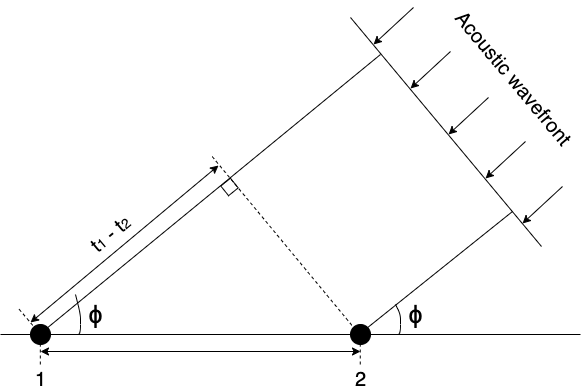
\includegraphics[width=0.7\textwidth]{figures/plane-wavefront}}
	\captionsetup{justification=centering,margin=2cm}
	\caption{Angle of arrival relation considering a plane wavefront}
	\label{fig:plane-wavefront}
\end{figure}

The estimator considers a USBL system composed by four sensors whose positions are previously defined. The time of arrival, $t_i$, to each hydrophone, $i$, is represented by expression (\ref{eq:toa-planewave}). The considered $t_0$ is the absolute time of emission of the signal, which is acquired through a synchronization mechanism, the $s$ is the position of the transmitter, $a$ is referent to the mass center of the USBL's position, $r_i$ is the Cartesian coordinates of the hydrophone's position, $c_s$ is the sound speed and $e_i$ is an injected error that have the same characteristics expressed previously in \ref{sec:premises}.

\begin{eqnarray}
& t_i = t_0 + \frac{ ||s - (a - r_i)|| }{c_s} + e_i
\label{eq:toa-planewave}
\end{eqnarray}

Due to the considered approximation to the plane wavefront, it is possible to estimate the range, $\rho$, as a mean all propagation times multiplied by the sound speed, $c_s$, as in equation (\ref{eq:range-planewave}). The $N$ represents the number of hydrophones.

\begin{eqnarray}
& \rho = c_s\ \frac{1}{N} \displaystyle\sum_{i=1}^{N} t_{i} - t_0
\label{eq:range-planewave}
\end{eqnarray}

Then a matrix $S$ is formulated as (\ref{eq:S}), whose rows are the difference between the position of hydrophone $i$ and the remaining three, and a $\Delta$ vector is expressed as (\ref{eq:delta}), containing all combinations of TDOA between hydrophone $i$ and the remaining.

\begin{eqnarray}
	& S = 
	\begin{bmatrix}
		r_i - r_j \\
		\cdots 
	\end{bmatrix}
	\label{eq:S}
\end{eqnarray}

\begin{eqnarray}
	& \Delta = 
	\begin{bmatrix}
		t_i - t_j \\
		\cdots 
	\end{bmatrix}
	\label{eq:delta}
\end{eqnarray}

Taking into account the defined $S$ and $\Delta$, the signal's angle of arrival can be calculated from the direction of the signal, $\tilde{d}$, obtained from the least squares expression (\ref{eq:direction-plane-wavefront}) \cite{estim-plane-wavefront}. Since there are only three equations to estimate three coordinates, then the expression is linear. It is important to notice that $(S^TS)$ has to be invertible, thus the rows which contain the chosen hydrophone configuration have to be linearly independent.

\begin{eqnarray}
& \tilde{d} = c_s \; (S^{T}S)^{-1} \; S^{T} \Delta
\label{eq:direction-plane-wavefront}
\end{eqnarray}

Having calculated the range $\rho$, given by the mean of the $rr_i$ magnitudes in figure \ref{fig:AoA-init}, and the direction $\tilde{d}$, the estimate of the transmitter position is given by the multiplication of these variables.

Finally, the plane wavefront estimator was integrated in a Monte Carlo method in order to execute multiple estimations of various transmitter positions, $s$, for a specific sensor configuration, so that it is possible to draw conclusions on its performance.

%------------------------------------------------------------------------------------
%-------------------------------------------------------------------------------------
\section{Fisher Information Matrix} \label{sucsec:FIM}

The Fisher Information Matrix (FIM) serves to quantify the information that an observable variable is capable of returning to an estimator. This concept is intrinsically linked with the Crámer-Rao lower bound \cite{bishop-cramer-rao}, which is a method that expresses the variance lower bound that a sensor configuration is capable of achieving, i.e. the best possible estimation precision it can achieve. Unlike the two previously presented processes, the Crámer-Rao bound is independent from the used estimator, as it assumes a linear estimator that is efficient and unbiased.

The fundamental process and mathematical notation previously used in \ref{sec:cramer} are applied in the procedure that will be explained next.

Firstly, the observation vectors are formulated based on an time of emission $t_0$, and the time of arrival based on the vectors that connect the hydrophone positions, $r_i$, to the transmitter, $s$. It is also considered an added noise component $e_i$, as defined in \ref{sec:premises}. The observations vectors are then expressed as (\ref{eq:obs-my}).

\begin{eqnarray}
	t_i = t_0 + \frac{s - r_i}{c} + n_i 
	\label{eq:obs-my}
\end{eqnarray}

Then, all conditions are set to calculate the FIM,  $I(d) \in \mathbb{R}^{3x3}$. In order to do so, if d$_{i}$ = $|| s - r_{i} ||$ is the distance between each sensor and the source, the gradient of the observations vector can be expressed as shown in (\ref{eq:grad_fisher}).

\begin{eqnarray}
	\nabla_{d}t(d) = \frac{1}{c} 
	\begin{bmatrix}
		\frac{d_1^T}{||d_1||} \\ 
		\addlinespace
		\frac{d_2^T}{||d_2||} \\
		\vdots \\
		\addlinespace
		\frac{d_N^T}{||d_N||}
	\end{bmatrix}
	\label{eq:grad_fisher}
\end{eqnarray}

Additionally, the added noise component is present in the covariance matrix, represented as (\ref{eq:covariance}), which integrates the FIM equation.

\begin{eqnarray}
	& \Sigma = 
	\begin{bmatrix}
		\sigma_1^2 & 0 & 0 & 0 \\
		0 & \sigma_2^2 & 0 & 0 \\
		0 & 0  & \sigma_3^2  & 0 \\
		0 & 0 & 0 & \sigma_4^2 
	\end{bmatrix}
	\label{eq:covariance}
\end{eqnarray}

Overall, the conditions to obtain the FIM matrix are established and, after some algebraic manipulations, it can be expressed as (\ref{eq:final-fisher}). This function can be validated by a similar study made on TOA based optimal positioning \cite{cramer-bruno}.

\begin{eqnarray}
	I(d) = \frac{1}{c^2} 
	\begin{bmatrix}
		\sum_{n=1}^{N} \frac{d_i d_i^T}{||d_i||^2} \frac{1}{\sigma_i^2}\\
	\end{bmatrix}
	\label{eq:final-fisher}
\end{eqnarray}

The final step is to calculate the determinant and find its relation to the volume of the \textit{uncertainty ellipsoid}. As mentioned in \ref{sec:cramer}, the determinant of the FIM returns a deterministic value that represents the quantity of information that can be obtained for a certain position, therefore, the objective is to maximize $det(I(d))$.

The FIM can be associated with a physical meaning, more specifically an uncertainty volume that characterizes the variance that a specific configuration can achieve for an estimate. In an initial approach, the ellipsoid was not considered and instead it was approximated to an uncertainty sphere with the same volume. The radius of the uncertainty sphere, $u_{sphere}$, is expressed as (\ref{eq:det-sphere}). In this situation, the optimization objective is to minimize the uncertainty radius.

\begin{eqnarray}
	& u_{sphere}(d) = \sqrt[2]{\sqrt[3]{det(I(d)^{-1})}}
	\label{eq:det-sphere}
\end{eqnarray}

In a further analysis, the length of the axis of the uncertainty ellipsoid are calculated using (\ref{eq:det-ellip}). The squared eigenvalues of the inverse of the FIM indicate the length of each of the three ellipsoid axis and the eigenvectors specify the direction of each axis. An eigenvector that is associated with the smaller eigenvalue indicates the direction in which there is less uncertainty and, equivalently, an eigenvector whose eigenvalue is the larger represents the direction in which there is the biggest uncertainty. Consequently, the goal in this case is to minimize the uncertainty ellipsoid axis that corresponds to the maximum uncertainty.

\begin{eqnarray}
	& u_{ellipsoid}(d) = \sqrt[2]{eig(I(d)^{-1})}
	\label{eq:det-ellip}
\end{eqnarray}

There are several optimality criteria that can be applied with the FIM in order to evaluate the estimation performance of a sensor configuration. Therefore, the selected metrics should be based on the intended application.
%----------------------------------------------------------------------------
%----------------------------------------------------------------------------

\section{Performance Comparison Between Methods} \label{subsec:perform-compar-meth}

Upon presenting the theoretical details behind the three considered methods for evaluating configurations' performance, a further functional study will be presented through simulation results. 

Throughout the functional demonstrations, three different hydrophone configurations are considered, A, B and C defined in \ref{tab:configs_test1}, where the columns $r_{Ai}$, $r_{Bi}$ and $r_{Ci}$ contain the position's coordinates of each hydrophone $i$.

\begin{table}[!htbp] %use H to adjust
	\begin{center}
		\begin{tabular}{ l | c c c c | c c c c | c c c c}
			%\hline
			%\multicolumn{1}{c|}{} & \multicolumn{4}{c|}{A} & \multicolumn{4}{c|}{B} \\
			\toprule
			% \cline{2-9}
			\multicolumn{1}{c|}{} & $r_{A1}$ & $r_{A2}$ & $r_{A3}$ & $r_{A4}$ & $r_{B1}$ & $r_{B2}$ & $r_{B3}$ & $r_{B4}$ & $r_{C1}$ & $r_{C2}$ & $r_{C3}$ & $r_{C4}$ \\
			\midrule
			\multirow{1}{0.5em}{x} 
			& 0.02 & 0.02 & 0 & 0 & 0.1 & 0.1 & 0 & 0 & 0.1 & 0 & 0 & 0  \\
			%\hline 
			\multirow{1}{0.5em}{y} 
			& 0 & 0 & 0.1 & -0.1 & 0 & 0 & 0.1 & -0.1 & 0 & 0 & -0.0707 & 0.0707 \\
			%\hline 
			\multirow{1}{0.5em}{z} 
			& 0.1 & -0.1  & 0 & 0 & 0.1 & -0.1  & 0 & 0 & 0 & 0.1 & -0.0707  & -0.0707\\
			\bottomrule 
		\end{tabular}
		\caption{Hydrophone configurations used for precision tests}
		\label{tab:configs_test1}
	\end{center}
\end{table}

In order to evaluate the performance of the configurations for the different methods, different criteria are considered, since the estimators and the FIM do not share the same evaluation metrics:

\begin{itemize}
	\item \textbf{Evaluation criteria used for GBE and PWE}
	
	To illustrate a scenario where these estimators are applicable, we can consider that a vehicle is moving towards an acoustic signal transmitter whose position is unknown. Imagining that the target is at a minimum of few meters, then the main focus is to achieve an optimal bearing estimation which provides a more direct path and saves resources. The range estimation serves as secondary measurement that indicates how near the vehicle is from the destination, so that it is possible to make control decisions such as moderate the navigation speed in the proximity of the target. For the reasons outlined, the study that follows presents a more thorough analysis of the azimuth and elevation errors. 
	
	For testing both estimators, a methodology was formulated in order to evaluate the precision that they achieve in defined circumstances. This approach is a Monte Carlo algorithm which allows to reiterate the estimation process according to the number of positions that are intended to be tested for a specific configuration, as well as create a series of repetitive calculations that allow to deduce the estimation error and turn the overall process more robust.
	%-------------
	The algorithm can be described as follows. For every defined position of the acoustic source, $s$, a function, that consists on the estimator, is called receiving as input the $s$, the positions of the hydrophone configuration, $r_i$, and an injected error $e_i$ of $0.5 \mu s$, that affects the ToA as detailed in \ref{sec:premises}. It then returns the estimated position of the source in Cartesian coordinates, $s_{cart}(x,y,z)$, and in spherical coordinates, $s_{sph}(n, \phi, \theta)$. As the position $s$ in Cartesian corresponds to the real value that is intended to be estimated, we can also obtain the real spherical coordinates by directly converting $s$ using the Cartesian to spherical relations in (\ref{eq:cart2sph}).
	
	\begin{eqnarray}
		\begin{cases} 
			n =  \sqrt{x^2 + y^2 + z^2}\\ 
			\phi  = arctan \frac{y}{x}\\ 
			\theta =  arctan \frac{\sqrt{x^2+y^2}}{z}
		\end{cases}
		\label{eq:cart2sph}
	\end{eqnarray}
	
	Consequently all conditions are met to analyze the achieved error in each coordinate by comparing the real position to the estimated values as (\ref{eq:error1}), where the observed coordinates are $n, \phi$ and $\theta$.
	
	\begin{eqnarray}
		&error_{coordinate} = |estimated_{coordinate} - real_{coordinate}|
		\label{eq:error1}
	\end{eqnarray}

	Additionally, the Mean-Squared Error (MSE) is also calculated in the spherical coordinates domain, which combines all errors in a single measurement.
	
	\item \textbf{Evaluation criteria used with the FIM}
	
	Several different optimality criteria can be applied using the FIM. Considering similar applications in literature \cite{optimality-e-a-d}, the evaluated criteria in the present work are the A-optimality, D-optimality and E-optimality, which are defined as follows:
	
	\begin{itemize}
		\item \textbf{A-optimality}: minimizes the trace of the inverse of the FIM, therefore seeks the minimum average variance of the estimates.
		\item \textbf{D-optimality}: minimizes the determinant of the inverse of the FIM, therefore the volume of the uncertainty ellipsoid. However, this can be misleading since the uncertainty in one direction can be much larger than the other directions, constituting a large FIM determinant which is not representative of the full estimation \cite{d-opt-mislead}.
		\item \textbf{E-optimality}: minimizes the largest eigenvalue of the inverted FIM, i.e. the ellipsoid axis with largest uncertainty. Since this criterion intends to minimize the axis that leads to the lower localization precision, then it is considered to be the most relevant in the present case (\textbf{RQ2}).
	\end{itemize}
	
\end{itemize}

Upon defining the general simulation conditions, there are two types of simulations that will be performed :
\begin{itemize}
	\item \textbf{Type SS (Specific Simulation)}, which is presented in this subsection, that compares the obtained performance result for each presented method when using a single configuration to estimate a specific transmitter position.
	\item \textbf{Type BS (Broad Simulation)} that tests the estimation of several positions with varying ranges, that form spheres around the origin of the coordinate axes, using multiple configurations for each of the methods.
\end{itemize}

\subsection{SS Analysis}

For the SS simulation, configuration C is used and the estimated position is $s_{cart}(100,0,0)$. Figures \ref{fig:SS-estimA-C-100,0,0}, \ref{fig:SS-estimB-C-100,0,0} and \ref{fig:SS-fim-C-100,0,0} correspond to the estimate dispersion obtained for each of the previously presented methods. The green point in each plot represents the position that is being estimated. As indicated the first plot represents the side view, plane zx, and the third plot is the view from above, plane yx, which illustrate the norm error, the second plot represents the USBL front view, plane zy, which corresponds to the error in azimuth and elevation angle.

As can be observed, the estimate dispersion obtained with GBE demonstrates a larger deviation in norm estimation than the other methods, of about $4m$. Additionally, it is observed in the front view an azimuth deviation of approximately $2.3^{\circ}$ and an elevation deviation of approximately $1.2^{\circ}$.

\begin{figure}[!htbp]
	\makebox[\textwidth][c]{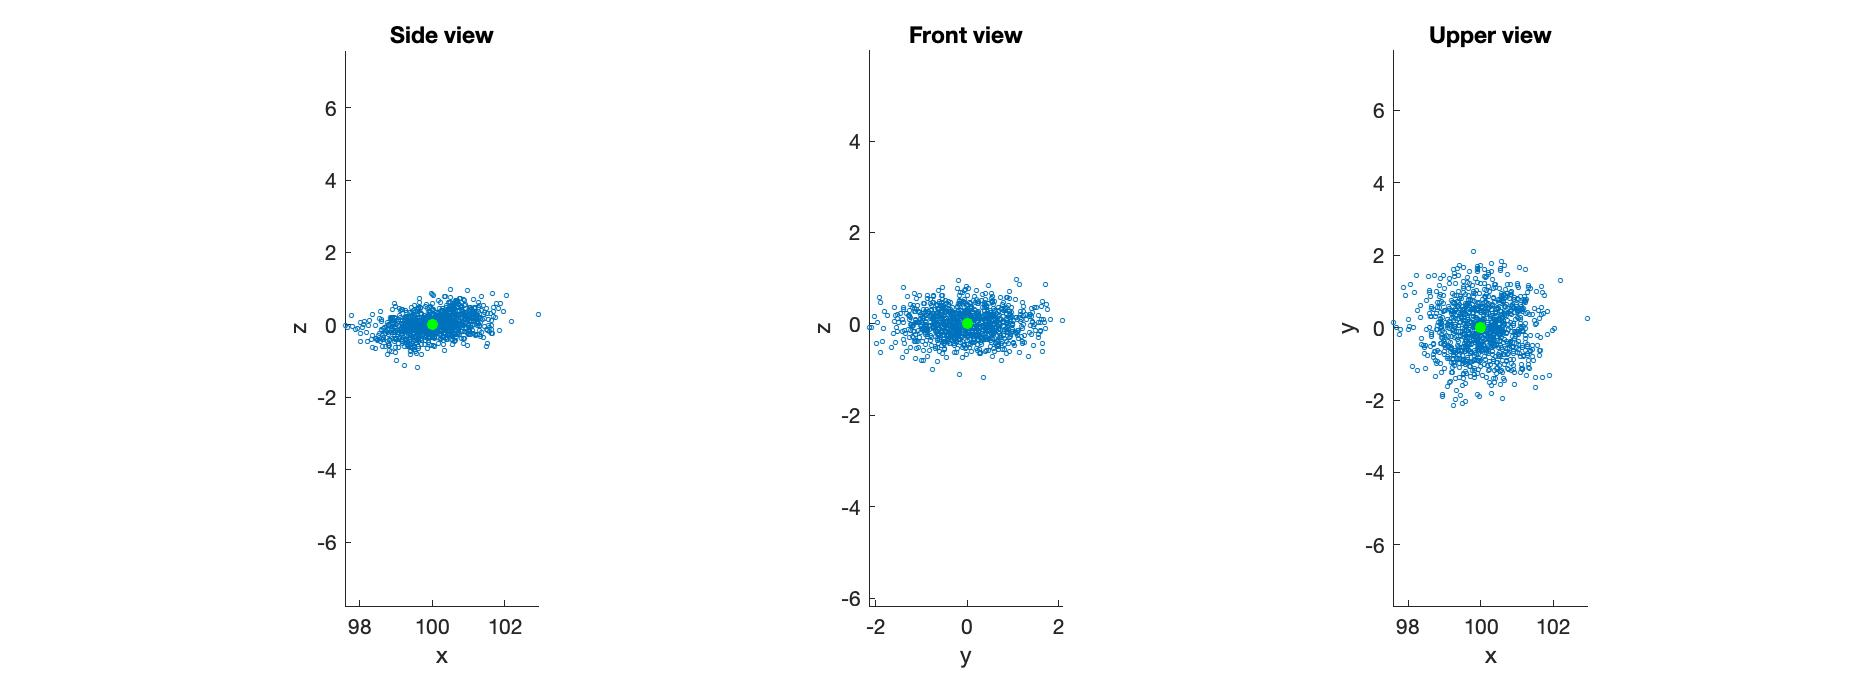
\includegraphics[width=1.4\textwidth]{figures/plot-compare-[100,0,0]-1279-1000s-estimA}}
	\captionsetup{justification=centering,margin=2cm}
	\caption{Estimate dispersion obtained with GBE for position $s_{cart}(100,0,0)$ using configuration C}
	\label{fig:SS-estimA-C-100,0,0}
\end{figure}

The PWE presents the estimate dispersion along a spherical surface, as expected since the method computes an average range. The norm estimation presents no significant deviation and the azimuth and elevation estimates show a similar dispersion as GBE.

\begin{figure}[!htbp]
	\makebox[\textwidth][c]{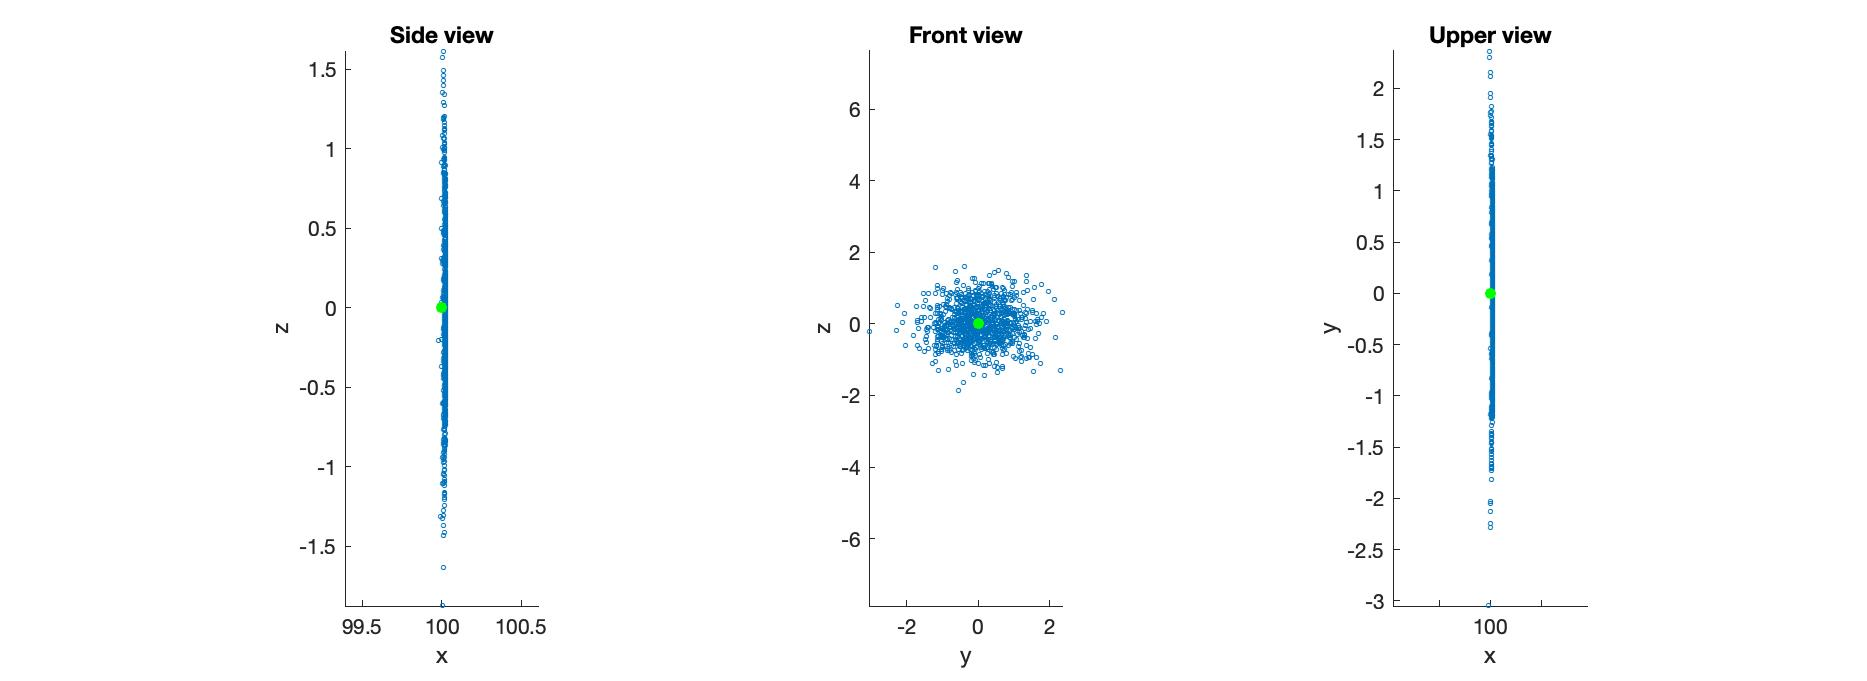
\includegraphics[width=1.4\textwidth]{figures/plot-compare-[100,0,0]-1279-1000s-pseudorange}}
	\captionsetup{justification=centering,margin=2cm}
	\caption{Estimate dispersion obtained with PWE for position $s_{cart}(100,0,0)$ using configuration C}
	\label{fig:SS-estimB-C-100,0,0}
\end{figure}

The FIM plot presents the expected uncertainty axis obtained for the specific position estimation. From the three methods it presents the smallest uncertainty in all three coordinates, with a deviation of $0.21^{\circ}$ in azimuth and $0.16^{\circ}$ in elevation.


\begin{figure}[!htbp]
	\makebox[\textwidth][c]{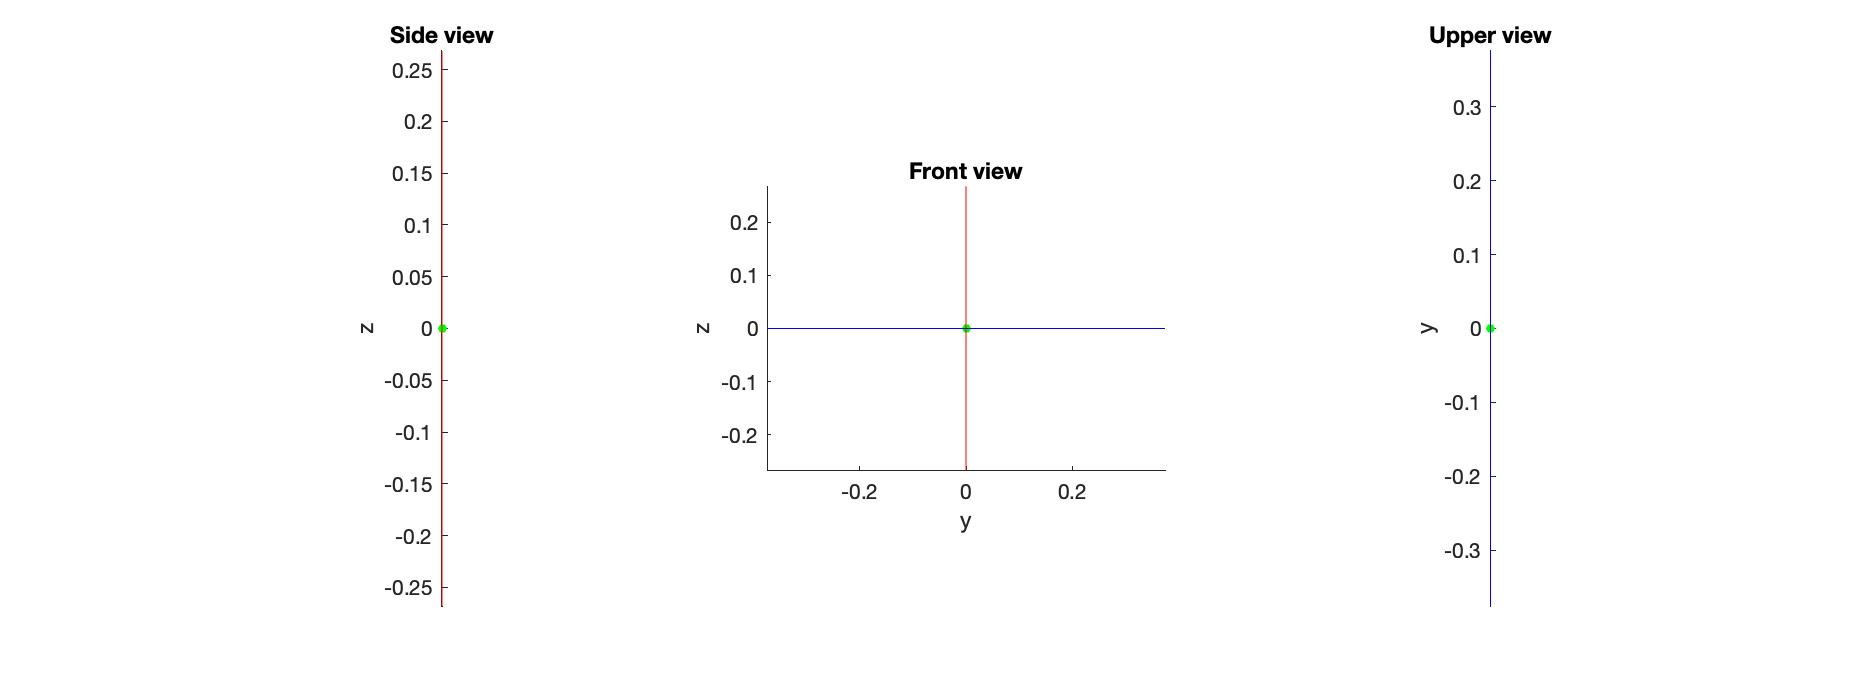
\includegraphics[width=1.4\textwidth]{figures/plot-fim-[100,0,0]-C}}
	\captionsetup{justification=centering,margin=2cm}
	\caption{Estimate dispersion obtained with FIM for position $s_{cart}(100,0,0)$ using configuration C}
	\label{fig:SS-fim-C-100,0,0}
\end{figure}

Overall, for a position situated at a distance of $100m$ the PWE method achieves a estimate dispersion format similar to the FIM in terms of norm estimation and an approximately equivalent dispersion to the GBE in terms of azimuth and elevation deviation.

\subsection{BS Analysis}

In the BS, the considered positions for the acoustic source, $s$, are originally defined in spherical coordinates, $s_{sph}$. These positions are arranged so that for each defined norm, the elevation component covers the interval [-90$^{\circ}$ , 90$^{\circ}$] in steps of one and, for each elevation value, the azimuth component covers the interval [-180$^{\circ}$ , 180$^{\circ}$] in steps of one, forming partial spheres around the reference axis' origin.

Then for each method, configurations A, B and C are tested for norms equal to $1m$ and $1000m$, that represent short and long range respectively. From each simulation using the estimators, the collected metrics are:
 
\begin{itemize}
	\item \textbf{Mean squared error} (MSE): Incorporates both the variance and the bias of the estimator;
	
	\item \textbf{Standard deviation of the error} ($\sigma$): Indicates how disperse are the estimates from the expected value;
	
	\item \textbf{Maximum error}: Indicates the maximum error that is obtained by the estimator, thus the worst precision achieved.
\end{itemize} 

Since the Crámer-Rao lower bound does not contemplate the azimuth and elevation errors as an optimality criteria, then other metrics are used in this case, which are the A-, D- and E-optimality, explained in \ref{sucsec:FIM}. Therefore, from all the tested positions, the collected measurements correspond to the following parameters: 

\begin{itemize}
	\item \textbf{Max Determinant}: Denotes the maximum uncertainty volume achieved for a specific position;
	
	\item \textbf{Determinant Standard Deviation}: Indicates the standard deviation of the ellipsoid uncertainty volumes computed for all positions $s$;
	
	\item \textbf{Min Max Eigenvalue}: Indicates the smaller value from the larger uncertainty axis obtained for each position;
	
	\item \textbf{ Min Trace}: Denotes the minimum sum of the uncertainty axes magnitudes
\end{itemize} 

Tables  \ref{tab:tdoa-estimator-abc}, \ref{tab:planewave-estimator-abc} and \ref{tab:fim-abc} summarize the collected data using the GBE, the PWE and the FIM, respectively.

\begin{table}[!htbp] %use H to adjust
	\begin{center}
		\makebox[\textwidth]{
			\begin{tabular}{ c | c c | c c | c c}
				%\hline
				\toprule
				\multicolumn{3}{c|}{} & \multicolumn{2}{c|}{Azimuth} & \multicolumn{2}{c}{Elevation}  \\
				\midrule
				\multicolumn{1}{c|}{Configuration} & Norm & MSE & Standard Dev & Maximum & Standard Dev & Maximum \\
				
				\midrule
				\multirow{2}{*}{A} &1 & 0.767 & 0.841 & 10.102 & 0.259 & 1.954\\
				&1000 & 0.759 & 0.751 &  9.243& 0.255 & 1.879\\
				
				\midrule	
				\multirow{2}{*}{B} &1 & 0.197 & 0.183 &  2.206 & 0.059 & 0.376\\
				&1000 & 0.199 & 0.186 & 2.186 & 0.061 & 0.368\\
				
				\midrule			
				\multirow{2}{*}{C} 
				&1 & 0.201 & 0.184 & 2.277  & 0.061 & 0.412 \\
				&1000 & 0.232 & 0.215 & 2.334 & 0.071 & 0.438\\
				\bottomrule 
		\end{tabular}}
		\caption{Obtained errors for configurations A,B and C by GBE}
		\label{tab:tdoa-estimator-abc}
	\end{center}
\end{table}

\begin{table}[!htbp] %use H to adjust
	\begin{center}
		\makebox[\textwidth]{
			\begin{tabular}{ c | c c | c c | c c}
				%\hline
				\toprule
				\multicolumn{3}{c|}{} & \multicolumn{2}{c|}{Azimuth} & \multicolumn{2}{c}{Elevation}  \\
				\midrule
				% \cline{2-9}
				\multicolumn{1}{c|}{Configuration} & Norm & MSE & Standard Dev & Maximum & Standard Dev & Maximum \\
				\midrule
				\multirow{2}{*}{A} 
				&1	& 9.547 & 15.054 & 169.741 & 3.228 & 16.542 \\
				&1000 &  2.111 & 14.277 & 37.660 & 3.461 & 7.665 \\
				\midrule	
				\multirow{2}{*}{B} 
				&1	& 2.233 & 1.054 & 8.546 & 0.690 & 3.708 \\
				&1000 & 0.582 & 0.561 & 6.581  & 0.204 & 1.740 \\
				\midrule			
				\multirow{2}{*}{C} 
				&1	& 1.982  &  1.887 & 20.133 & 0.624 & 3.584 \\
				&1000 & 0.726 & 0.642 & 9.855 & 0.218 & 2.029\\
				\bottomrule 
		\end{tabular}}
		\caption{Obtained errors for configurations A,B and C using PWE}
		\label{tab:planewave-estimator-abc}
	\end{center}
\end{table}

\begin{table}[!htbp] %use H to adjust
	\begin{center}
		\makebox[\textwidth]{
			\begin{tabular}{ c | c | c c | c | c }
				%\hline
				\toprule
				\multicolumn{2}{c|}{} & \multicolumn{2}{c|}{Determinant} & \multicolumn{1}{c|}{Max Eigenvalue} & \multicolumn{1}{c}{Trace}  \\
				
				\midrule
				\multicolumn{1}{c|}{Configuration} & Norm & Max & Standard Dev & Min & Min\\
				
				\midrule
				\multirow{2}{*}{A} 
				& 1 	 & 4.2$\times10^{-3}$ & 6.65$\times10^{-4}$  & 5.3$\times10^{-3}$ & 5.60$\times10^{-5}$  \\
				%& 10 	 & 0.010 & 0.0200 & 0.003 & 0.053 & 5.6$\times10^{-3}$  \\
				& 1000 & 0.421 & 0.067 & 5.310 & 56.325 \\
				
				\midrule	
				\multirow{2}{*}{B} 
				& 1 	  & 2.5$\times10^{-3}$ & 8.78$\times10^{-5}$& 5.3$\times10^{-3}$ & 5.17$\times10^{-5}$  \\
				%& 10 	 & 0.010 & 0.011 & 3.8$\times10^{-4}$ & 0.0530 & 5.6$\times10^{-3}$ \\
				& 1000 & 0.2462 & 0.008 & 5.306 & 56.283 \\
				
				\midrule			
				\multirow{2}{*}{C} 
				& 1 	 & 3.0$\times10^{-3}$  & 1.39$\times10^{-4}$  & 7.1$\times10^{-3}$ & 8.42$\times10^{-5}$  \\
				%& 10 	 & 0.012  & 0.014 & 6.3$\times10^{-4}$ & 0.075 & 8.5$\times10^{-3}$  \\
				& 1000 & 0.290 & 0.014 & 7.410 & 84.882 \\
				\bottomrule 
		\end{tabular}}
		\caption{Obtained errors for configurations A,B and C by Crámer-Rao lower bound}
		\label{tab:fim-abc}
	\end{center}
\end{table}

By inspection, it is possible to observe that for both the GBE and PWE, the maximum deviations are considerably distant from the standard deviation, which correspond to positions in space with elevation values around $-90^{\circ}$ and $90^{\circ}$ where it is achieved the worse estimation precision. Furthermore, while the minimum deviations in both estimators are similar, the PWE reveals much larger maximum errors since there are regions of space for which its localization precision is much lower. 

Regarding the PWE, it should also be noted that the obtained standard deviations for short range of $1m$ are visibly higher than for long range of $1000m$, as expected since the approximation to the plane wavefront is only valid for long distances.

Finally, as the Crámer-Rao lower bound contemplates the best possible estimation precision for a sensor configuration, then the collected values for this case are consequently lower than the previous methods. 

\subsection{Behavioral Analysis}

Having analyzed the performance of the studied methods, there are still two factors that can be explored in order to further understand its impact on the estimation precision.  The first idea explores the impact of the the ToA measurement on the position estimation and the second studies the influence of an increasing baseline of the geometric configuration on the estimation precision.

\subsubsection{Impact of ToA measurement on position estimation}

As previously mentioned, the GBE uses the approximation which allows all hydrophones to use the a reference ToA added by a TDoA, representing the total time it takes for a signal to travel between the transmitter and each hydrophone. However, for long range positions the ToA is consequently much larger in relation to the time differences of arrival. So, the hypothesis is that for these cases the ToA is irrelevant for the calculations so it can be discarded. Therefore, for the angle of arrival estimation it is only necessary to use the TDoAs.

In order to simulate this, the reference time ToA is substituted by $\frac{10^4 m}{1500 m/s}$, which corresponds to a distance of $10 km$. The results demonstrated no visible change in the error of the estimate. However, for distances bellow $100m$ the impact of this approximation is noticeable. Therefore, it is considered that the hypothesis is valid. 

\subsubsection{Influence of increasing the configuration baseline}

In this research work, the configuration baseline corresponds to the geometric distance between hydrophones. Until this point, there are several obtained results which demonstrate the influence of the used baseline on the estimation performance. However, there are no conclusions about the optimal baseline length that should be used. The goal of this test is to delineate the influence of increasing the hydrophones' baseline in the obtained error. 

In order to execute this test, the GBE is used with configuration C. To create an increasing baseline along the tests, in each iteration the $x$ coordinate of $r_{C1}$ increases $0.01 m$ in a total of 200 times, which makes up a displacement range between 0.1 and $2 m$. Each position generates 100 accumulated samples that result in a single measurement per configuration. 

Plot \ref{fig:plot-baseline-increase-1} represents the collected errors for each of the described configurations, whose baseline is progressively increasing in a constant pace. As illustrated, the obtained errors decrease visibly in the first 100 tests, corresponding to a $r_{C1}$ position between 0.1 and $1 m$, becoming considerably constant for further distances.

\begin{figure}[!htbp]
	\makebox[\textwidth][c]{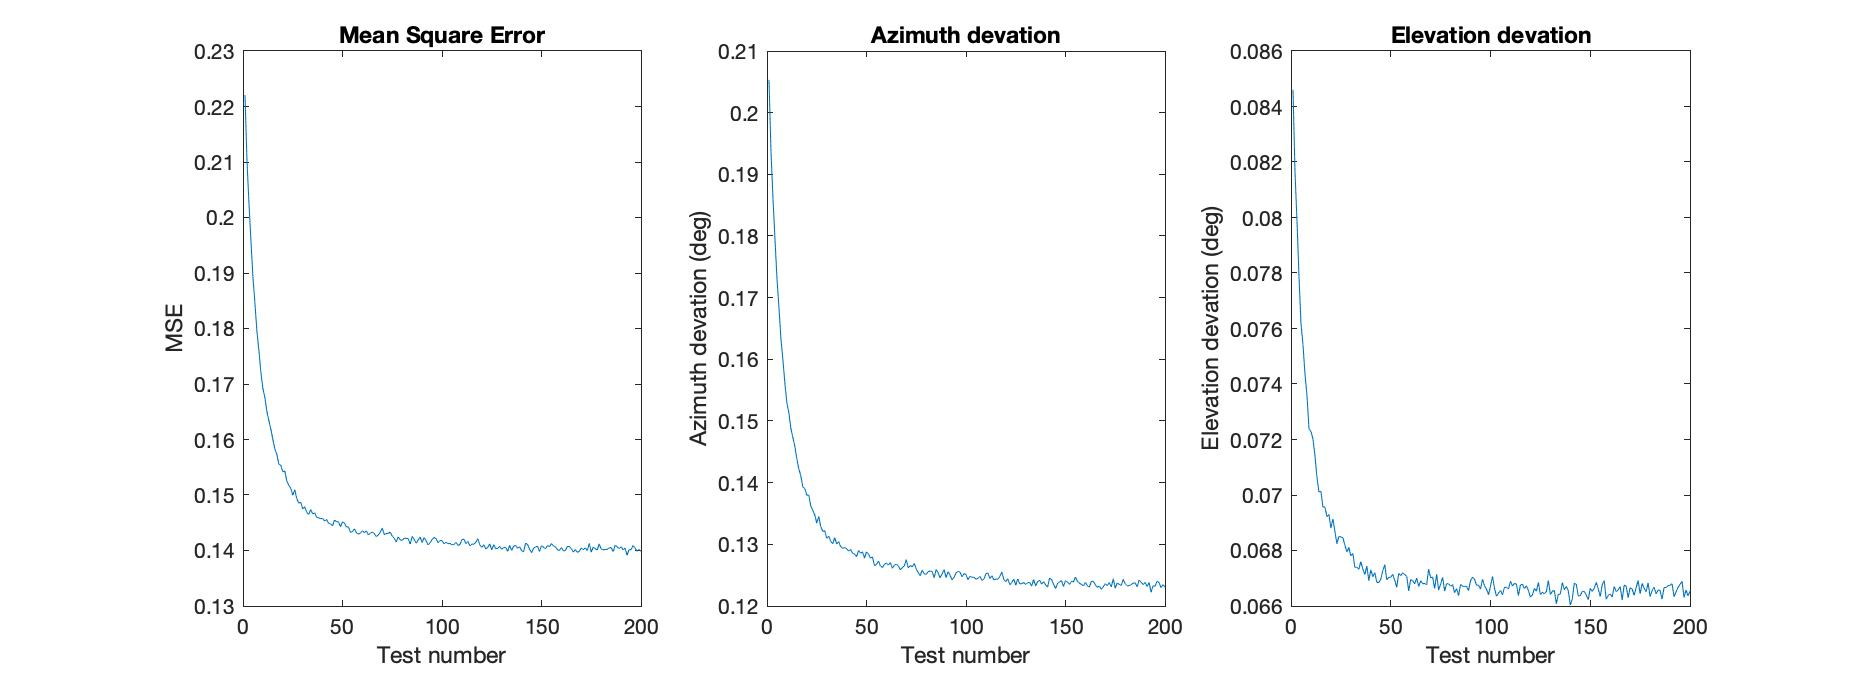
\includegraphics[width=1\textwidth]{figures/plot-Hbaseline-dev001-100accum-100s-1}}
	\captionsetup{justification=centering,margin=2cm}
	\caption{Error evolution with increasing baseline for $r_{C1}$}
	\label{fig:plot-baseline-increase-1}
\end{figure}

Additionally, the same experiment was done on hydrophone $r_{C2}$ of the same structure, since its position on the configuration gets a different exposure than $r_{C1}$ and a different outcome is expected. Having considered the same conditions as explained for the previous simulation, figure \ref{fig:plot-baseline-increase-2} illustrates the obtained results. It can be observed that the displacement of this specific hydrophone only causes an estimation improvement in the elevation deviation, it does not affect the estimation of the azimuth deviation and slightly increases the azimuth deviation. Therefore, an estimation improvement may not be achieved by distancing a random hydrophone, a study should be conducted for each particular configuration to determine which displacements lead to an enhancement.

\begin{figure}[!htbp]
	\makebox[\textwidth][c]{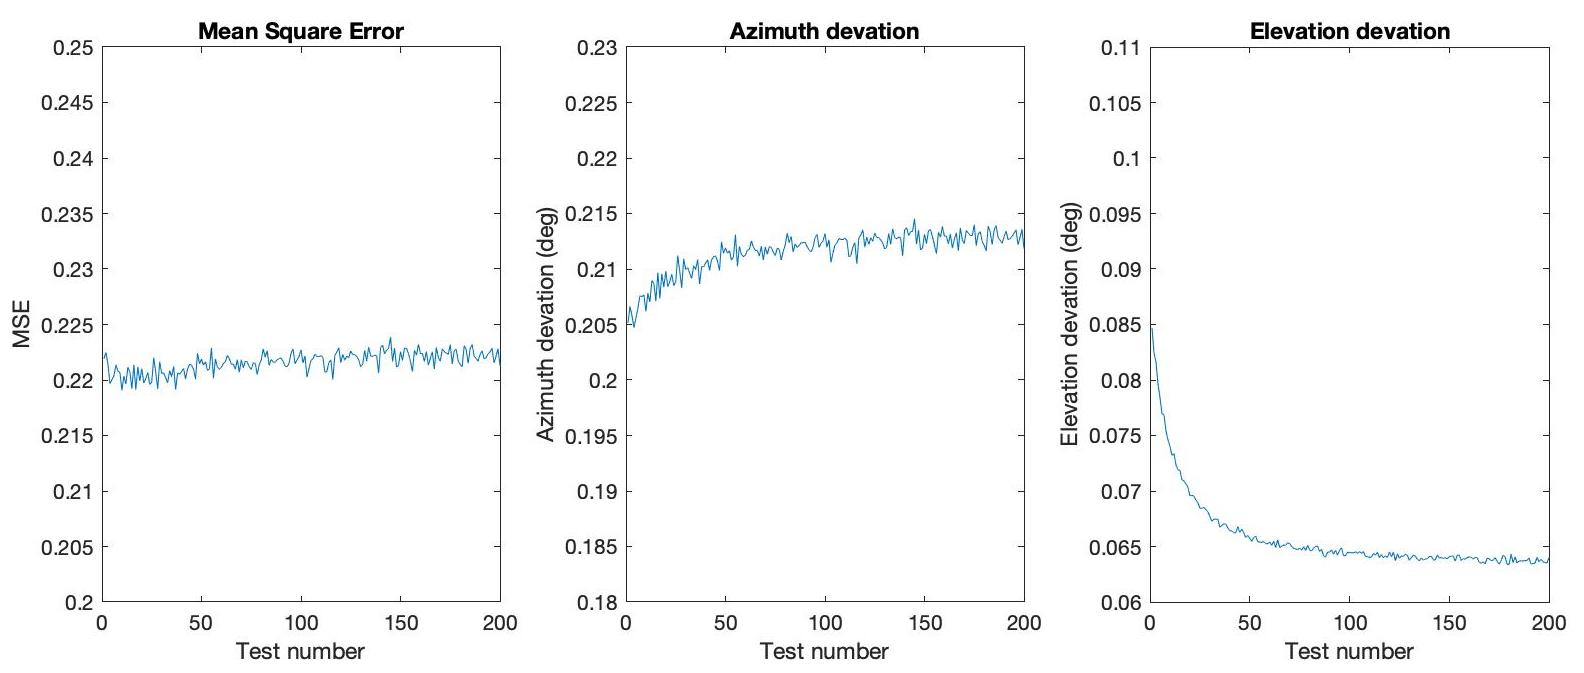
\includegraphics[width=1\textwidth]{figures/plot-Hbaseline-dev001-100accum-100s-2}}
	\captionsetup{justification=centering,margin=2cm}
	\caption{Error evolution with increasing baseline for $r_{C2}$}
	\label{fig:plot-baseline-increase-2}
\end{figure}

In conclusion, it is proved that increasing the baseline of a configuration in specific cases may result in a decrement of the overall estimation error. However, this only occurs for a maximum distance after which the error variation is not significant . 

\subsubsection{ Conclusions on behavioral analysis}

The present chapter focused on a further analysis of the impact of some system characteristics to the estimation, involving mechanisms based on simulated results. Therefore, by way of summary, some main conclusions can be taken:

\begin{itemize}
	\item As expected, the azimuth and elevation errors do not vary with the range of the transmitter's position, in contrast to errors in Cartesian coordinates which increase proportionally with the range;
	
	\item The ToA measurement is not essential for long range distances. So, in those cases it can be discarded decreasing the dependency on the synchronization mechanism;
	
	\item Increasing the baseline of a hydrophone configuration can result in a better estimation, until reaching a certain distance after which the error becomes constant. Therefore, when choosing an hydrophone layout which can be limited to the dimensions of a physical structure, it does not have to be sought the maximum baseline possible but the length that leads to an error variation not significant ;
	
	\item The hydrophone configuration is a main factor on the estimation performance for any position in space. Although the characteristics that a configuration should meet to be optimal are still not clear, some aspects can be pointed out: 
	
	\begin{itemize}
		\item It is mandatory to ensure a sensor layout which covers three dimensions, so it is possible to estimate coordinates in 3D;
		\item The positions of the sensors must not be coplanar to allow the application of the least squares method;
		\item It is fundamental to have an adequate baseline which can be determined with the tool previously explained, to avoid singularities on the estimators and obtain lower estimation errors;
		\item Bearing in mind that the configuration may be employed in real scenarios, it is useful to create schematics which require achievable distances between hydrophones and respect logical shapes to install in vehicles such as AUVs.
	\end{itemize}
\end{itemize}

\section{Final Remarks}

This section focuses on three selected methodologies that are capable of evaluating sensor configurations' performance based on multiple criteria.

From the presented methods, it is expected that for short range estimation, distances from few centimeters to few meters,  the GBE presents estimates that are more approximated to the real value than the PWE, since it uses the geometric relations between the hydrophone and the transmitter in order to estimate the position. Contrarily, for long range estimations, distances higher than a few meters, the PWE is expected to achieve lower estimation errors than the GBE, since it is a linear system and the approximation it considers does not affect the estimation.

Lastly, as the FIM reflects the quantity of information that a configuration is capable of acquiring in relation to a specific position, then it can be directly related to the precision of the estimation. The Crámer-Rao lower bound, which is intrinsically linked to the FIM, assumes the use of any unbiased and efficient estimator, which makes it a more generic tool. Consequently, it is widely used in literature for sensor configuration's performance analysis. 

In conclusion, due to the generality of the tool, the FIM is considered the most efficient tool for this application (\textbf{RQ1}). 
